\chapter{REVIEW OF LITERATURE AND STUDIES} %\label{cap:Chapter2}

%This chapter starts  with a brief introductory paragraph concerning the researcher’s exploration of related literature and studies on the research problem. It should be organized thematically to confirm to the specific problems. It should synthesize evidence from all studies reviewed to get an overall understanding of the state of the knowledge in the problem area. As much as possible, the reviewed should be limited within the last ten years. A statement showing how the related materials had assisted the researchers in the present study should be the last part.  

%This chapter discusses the literature studies and theories of this study. It is divided into two sections: (1) the related literatures; and (2) the related studies.


%**********************************************
%3.     Tinjauan Pustaka (pada Bab 2, judul Bab bukan Tinjauan Pustaka, disesuaikan dengan konten)
%Berisi landasan teori yang digunakan dalam penyelesaian tesis. Gunakan literature 3 tahun terakhir. Berisi minimal 3 halaman.
% =========================================================
%\section{Related Literatures}
% =========================================================
\section{Autonomous Trash Collector Robot}
%This section discusses state of the art of biometrics technologies and typical process which should be conducted in biometrics such as: data acquisition; preprocessing; feature extraction; and classification.
 
 Beberapa penelitian terkait Autonomous Robot untuk pengolahan sampah telah banyak dilakukan pada beberapa penelitian. Salah satunya pada penelitian yang dilakukan oleh Aditya P. P. Prasety, etc \cite{Prasetyo2020}, di mana pada penelitian tersebut Autonomous Robot dibuat menggunakan lengan manipulator untuk mengambil sampah. Posisi robot dikendalikan berdasarkan sensor ultrasonic dan sistem navigasi. Robot tersebut mampu membersihkan dua jenis sampah sebanyak 40 kali. Penelitian lain serupa juga dilakukan oleh Muhammad Abbas Khan, et al \cite{Khan2020}, dimana pada penelitian tersebut Robot Semi-autonomous dibuat untuk mengambil sampah berdasarkan perintah dari perangkat Smartphone melalui bluetooth. Robot juga dilengkapi sensor ultrasonic sehingga mampu mendeteksi posisi sampah. Pada Referensi \cite{Bai2018}, sebuah Autonomous Robot dibuat untuk mengambil sampah yang beroperasi di rumput. Robot mampu mendeteksi sampah secara otomatis dan akurat dengan menggunakan algoritma Deep Neural Network \cite{Kong2009}. Robot tersebut dilengkapi sensor ultrasonic\cite{Michael2008} dan sistem navigasi \cite{Wang2008}. Hasil pengujian menunjukan bahwa robot mampu mendeteksi sampah dengan akurasi 95\%. Pada makalah\cite{Arai2019}, Autonomous Robot dirancang menggunakan algoritma Convolutional Neural Network (CNN) untuk mendeteksi berbagai jenis sampah, seperti kaleng, botol plastik, dan kotak makan siang secara otomatis. Sistem robot mampu mendeteksi sampah secara outdoor. Berdasarkan data hasil pengujian\cite{Arai2019}, robot tersebut mampu mendeteksi sampah dengan tingkat kepresisian sebesar 95,6\% dan tingkat akurasi sebesar 96,8\% .


Pada penelitian ini akan dirancang sebuah autonomous mobile robot berjenis mobile robot beroda dengan menggunakan metode differential drive untuk pergerakan robot menuju obyek. Robot menggunakan kamera untuk mendapatkan citra  obyek (obstacle dan target), mendapatkan path planning dari hasil citra bola untuk pergerakan posisi robot.
% =========================================================
%\section{Related Studies}
% =========================================================
%This section discusses about the related studies which support in the designing of the proposed method.

\section{Autonomous Mobile Robot}
Robot yang sepenuhnya otonom dapat memperoleh informasi tentang lingkungan, bekerja untuk waktu yang lama tanpa campur tangan manusia, memindahkan semua atau sebagian dari dirinya sendiri di seluruh lingkungan operasinya tanpa bantuan manusia, menghindari situasi yang berbahaya bagi manusia, properti. Robot otonom juga dapat belajar atau mendapatkan pengetahuan baru seperti menyesuaikan metode baru untuk menyelesaikan tugasnya atau beradaptasi dengan lingkungan yang berubah. Oleh karena itu, robot bergerak perlu memiliki kemampuan otonomi dan kecerdasan, dan untuk merancang algoritme yang memungkinkan robot berfungsi secara mandiri di lingkungan yang tidak terstruktur, dinamis, sebagian dapat diamati, dan tidak pasti menimbulkan tantangan bagi para peneliti untuk menangani masalah kunci.
Masalah seperti ketidakpastian (baik dalam penginderaan dan tindakan), keandalan, dan respons waktu nyata.

Di masing-masing domain aplikasi mobile robot, mobilitas hampir tidak ada gunanya tanpa kemampuan bernavigasi. Gerakan acak, yang tidak memerlukan kemampuan navigasi, mungkin berguna untuk pengawasan atau operasi pembersihan tertentu, tetapi untuk sebagian besar aplikasi ilmiah atau industri robot bergerak, kemampuan untuk bergerak dengan cara yang bertujuan diperlukan. Oleh karena itu, navigasi otonom memainkan peran kunci dalam keberhasilan robot, dan juga dasar untuk teknologi relatif robot bergerak otonom.

\begin{figure}[H]
	\centering
	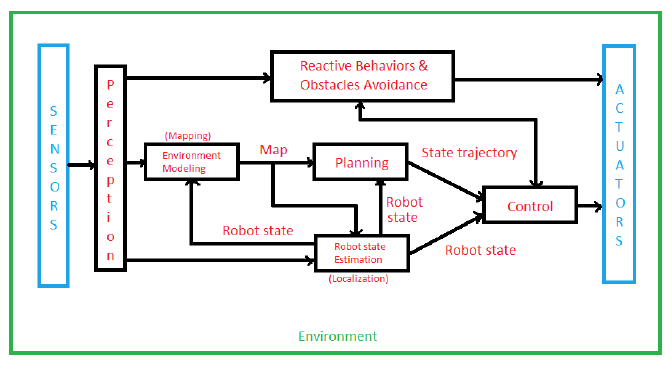
\includegraphics[width=0.7\linewidth]{figure/screenshot004}
	\caption{Autonomous Navigation System}
	\label{fig:screenshot004}
\end{figure}

Tugas navigasi mobile robot mengacu pada rencana jalur dengan penghindaran rintangan ke tujuan tertentu dan untuk melaksanakan rencana ini berdasarkan pembacaan sensor. Navigasi robot seluler secara kasar mencakup enam kompetensi yang saling terkait berikut ini \ref{fig:screenshot004}.  

\begin{enumerate}
	\item Perception: untuk memperoleh dan menginterpretasikan informasi sensorik;
	\item Exploration: strategi yang memandu robot untuk memilih arah selanjutnya;
	\item Mapping:untuk membangun representasi spasial atau model lingkungan dengan menggunakan informasi sensorik yang dirasakan;
	\item Localization: strategi untuk memperkirakan posisi robot dalam peta spasial yang terjadi secara bersamaan untuk kontrol navigasi;
	\item Path planning: strategi mencari jalur menuju lokasi tujuan yang optimal atau tidak;
	\item Path execution: untuk menentukan dan menyesuaikan aksi motorik dengan perubahan lingkungan, juga termasuk penghindaran rintangan.
\end{enumerate}

Sebuah robot membutuhkan mekanisme yang memungkinkan untuk bergerak bebas di lingkungan, yaitu, harus mampu mendeteksi dan bereaksi terhadap situasi. Ini adalah sensor robot yang memainkan peran seperti mata robot, dan robot tahu di mana itu atau bagaimana caranya ke suatu tempat, atau untuk dapat menjelaskan ke mana ia pergi. Sensornya bisa fleksibel dan mobile untuk mengukur jarak yang telah ditempuh roda sepanjang tanah, untuk mengukur perubahan inersia dan struktur eksternal di lingkungan.


%\subsection{Kinematika Differential Drive Mobile Robot}
%\subsection{Motor DC}
%\subsection{Driver Motor DC dan Pulse Width Modulation (PWM) }
% =========================================================
\section{Mobile Robot Control Architectures}
% =========================================================
Arsitektur kontrol robot bergerak melibatkan proses mengambil informasi tentang lingkungan melalui sensor robot, memprosesnya seperlunya untuk membuat
keputusan tentang bagaimana bertindak, dan pelaksanaan tindakan di lingkungan. Arsitektur kontrol tradisional (deliberatif) diturunkan dari paradigma kecerdasan buatan (AI) tradisional, di mana perencana pusat menggabungkan semua pembacaan sensor, membangun model dunia, merencanakan tindakan selanjutnya, dan akhirnya mengarahkan robot. Gambar \ref{fig:screenshot005} menggambarkan arsitektur tersebut. 
\begin{figure}[H]
	\centering
	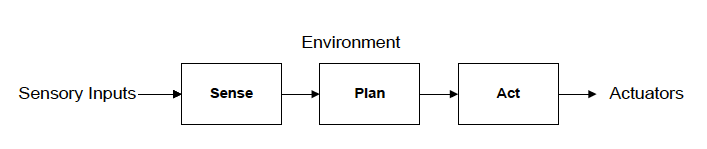
\includegraphics[width=0.7\linewidth]{figure/screenshot005}
	\caption[]{Traditional sense–plan-act architecture}
	\label{fig:screenshot005}
\end{figure}

Robot awal seperti Shakey [Nilsson, 1984] mengadopsi jenis arsitektur ini, yang pada intinya berusaha mengatasi ketidakpastian lingkungan dengan menciptakan model dunia.
Musyawarah mengacu pada berpikir keras, dan didefinisikan sebagai perhatian dalam mengambil keputusan dan tindakan [Nattharith, 2010]. Sistem kontrol umumnya diatur menggunakan dekomposisi fungsional dari proses pengambilan keputusan, yang terdiri dari beberapa modul untuk pemrosesan sensorik, pemodelan dan perencanaan, penilaian nilai, dan eksekusi [Brooks, 1986]. Dekomposisi fungsional seperti itu memungkinkan operasi kompleks untuk dilakukan, tetapi menyiratkan independensi berurutan yang kuat antara modul pengambilan keputusan. Arsitektur ini mampu bekerja dengan sukses dalam lingkungan yang terstruktur. Misalnya, jika ada cukup waktu untuk menghasilkan rencana dan model dunia akurat, pendekatan ini memungkinkan robot menghasilkan tindakan terbaik untuk situasi tertentu. 

Namun, seperti arsitektur cenderung gagal dalam lingkungan yang tidak terstruktur atau bahkan dalam lingkungan yang terstruktur secara longgar karena ketidakmampuan mereka untuk beradaptasi dengan lingkungan. Selain itu pendekatan tersebut terbatas dalam kegunaannya karena kurangnya reaktivitas waktu nyata, dan mungkin sepenuhnya gagal jika salah satu bagian gagal. Oleh karena itu arsitektur murni yang disengaja tidak lagi digunakan untuk sebagian besar robot bergerak fisik yang bekerja di lingkungan dunia nyata yang kompleks dan berubah secara dinamis [Peng, 2004; Natharith, 2010].

%\subsection{Reactive/Behaviour based architecture } 
%Pada akhir 1980-an, konsep robotika berbasis perilaku diperkenalkan di MIT AI laboratorium [Brooks, 1986]. Menurut paradigma ini, perilaku dasar, yang melibatkan motorik reaksi terhadap rangsangan sensorik, adalah blok bangunan dari perilaku yang lebih kompleks. Ini konsep meninggalkan ide perencana pusat yang memiliki pengetahuan yang komprehensif tentang sistem [Peng, 2004]. Pendekatan ini terinspirasi oleh gagasan biologis stimulusrespon, sehingga tidak bergantung pada jenis proses penalaran kompleks yang digunakan dalam arsitektur yang disengaja.
%Informasi diproses secara paralel daripada berurutan. Pada dasarnya, data sensorik didistribusikan ke modul reaktif individu. Masing-masing melakukan tugas tertentu seperti seperti menghindari rintangan atau mengidentifikasi tujuan. Sistem yang paling terkenal untuk berbasis perilaku kontrol adalah arsitektur subsumption, diperkenalkan oleh Rodney Brooks pada tahun 1985, [Brooks, 1986].
%\subsection{Subsumption architecture }
%Brook percaya bahwa robot pada dasarnya harus reaktif [Brooks, 1986]. Dalam arsitektur subsumsi, pendekatan berbasis perilaku memerlukan dekomposisi horizontal perencanaan menjadi kumpulan lapisan bersamaan; masing-masing terhubung ke input sensoriknya sendiri. Serangkaian perilaku mendefinisikan sistem kontrol. Perilaku diimplementasikan sebagai proses waktu nyata yang mengambil input dari sensor atau perilaku lainnya dan mengirim perintah keluaran ke efektor atau perilaku lainnya. Kontroler pada dasarnya adalah jaringan terdistribusi dari perilaku yang dieksekusi secara bersamaan. Contoh yang diberikan arsitektur diilustrasikan pada Gambar \ref{fig:screenshot006}. Sebuah arsitektur subsumption terdiri dari satu set lengkap sistem kontrol robot. Masing-masing mampu mencapai tingkat tertentu kompetensi. Desain arsitektur subsumption konvensional yang diusulkan oleh Brooks [1986] mendefinisikan delapan lapisan kompetensi yang diberi label dari 0 hingga 7.

%Namun hanya lapisan 0 sampai 2 yang telah diimplementasikan pada robot [Toal et al., 1995] . Lapisan 0 menyediakan kemampuan untuk menghindari rintangan, sedangkan Layer 1 memungkinkan robot untuk berkeliaran tanpa tujuan. Layer 2 memberi robot kemampuan untuk menjelajahi dunia dengan menggunakan sensornya dan menuju ke lokasi yang diamati. Lapisan 3 hingga 7 memerlukan lebih banyak perilaku yang kompleks, seperti kemampuan untuk memetakan lingkungan, merumuskan rencana tentang itu, dan alasan tentang keadaan dunia. Tim yang dipandu oleh Brooks melakukan beberapa penyelidikan awal tentang bagaimana perilaku tersebut dapat diimplementasikan dalam robot, tetapi masih belum jelas seberapa sukses hal ini dalam jangka panjang [Toal et al., 1995].
%Beberapa robot telah dirancang berdasarkan arsitektur subsumption. Contohnya: Allen - robot berbasis subsumsi pertama [Brooks, 1986], Tom and Jerry - dua kecil mobil mainan yang dilengkapi dengan sensor jarak inframerah [Brooks, 1990]; dan Toto – fokus pada konstruksi peta untuk robot berbasis subsumsi [Mataric, 1992]. Yang lebih baru implementasi arsitektur ini dirancang untuk menjalankan mobile robot di medan yang kasar, menggunakan pengenalan tengara visual yang cerdas dan penghindaran rintangan berbasis fuzzy [Li dan Yang, 2003]. Atau, arsitektur berbasis perilaku untuk menemukan dan melacak bahan kimia yang menggunakan arsitektur subsumption telah diimplementasikan untuk AUV [Wei dkk., 2006]. Di sisi lain, karena arsitektur ini hanya dapat menjalankan satu tugas pada a waktu, robot cepat atau lambat akan mengalami situasi di mana tindakan yang benar harus ditetapkan dengan menggunakan kombinasi perilaku. Misalnya, ketika robot menghindari rintangan saat bergerak menuju tujuannya, arsitektur subsumption akan memanggil perilaku menghindari sebagai prioritas sebelum perilaku goto. Robot mungkin menghindari rintangan dengan sukses, tetapi robot dapat menghindarinya dengan cara yang mengarahkannya jauh dari tujuannya. Itu karena tidak mampu mempertimbangkan beberapa perilaku yang secara signifikan dapat mengurangi kinerja [Hoffmann, 2003].

%\subsection{Motor schema} 
%nother important example of reactive based architectures is the motor schema proposed by Arkin [1987], as illustrated in Figure 2.5. Motor schemas are proposed as a basic unit of behaviour specification for the navigation of a mobile robot. They generate response vectors based on the outputs of the perceptual schemas. The schema has a fusion mechanism used to combine the response vectors generated in a manner similar to the Potential Field Method [Khatib, 1985]. According to this method, a goal is represented by an attractive force while obstacles are represented by repulsive forces.
%The summation of these force vectors is treated as the coordinated action for the robot to take to complete a particular task. However, the architecture has certain drawbacks. The most common is the local minima problem in which attractive and repulsive forces cancel each other out. Thus the overall sum is null and the robot cannot move from its current location. Various alternative solutions have been proposed to overcome this problem [Nattharith, 2010]. However, another problem with this architecture is that the action executed is, in essence, one that no behaviour has generated. For instance, consider a robot with an obstacle ahead. Assuming that two different behaviours generate outputs for avoiding that obstacle, one trying to avoid it to the right and the other one trying to avoid it to the left, then the sum of the vector would direct the robot straight ahead at the obstacle [Peng, 2004]. 	\label{fig:screenshot007}



%\subsection{Hybrid architecture} 
%While it has been widely demonstrated that behaviour based architectures effectively produce robust performance in dynamic and complex environments, they are not always the best choice for some tasks. Sometimes the task to be performed needs the robot to undertake some degree of deliberation and maintain a model of the environment.
%However, behaviour based architectures avoid this deliberation and modelling. Additionally, as mentioned previously, purely deliberative architectures are also not the best choice for tasks in complex environments. Thus, a compromise between these two completely opposite views must be reached. Hybrid architectures are composed of two parts, the first for deliberation and the other is the reaction part. The deliberation part allows the modelling of the world and creating plans, while the reactive part on the other hand is responsible for executing plans and quickly reacting to any unpredicted situation that may arise. Hybrid architectures are essentially structured in three layers.
%Because of the ability to combine the advantages of both deliberate and behaviour based systems, this approach has become important in designing mobile robot systems, and is considered to offer an appropriate solution for further development. For instance, Nattharith [2010] implemented a hybrid based architecture which is based upon the motor schema described above.




%\subsection{Object Detection}
%Object detection is a key task in fields of computer vision and robotics. Some object detection methods are well developed, such as feature analysis (Comaniciu \& Meer, 2002), segmentation(Sumengen et al., 2003), blob clustering (Ana \& Jain, 2003), object recognition (Lowe, 2004), and illumination invariance (Finlayson et al., 2001). Some well-developed image processing tools are integrated in OpenCV, Matlab etc. as libraries for usage. These libraries brought a lot of advantages to robotics. For example, some libraries in OpenCV include: template matching to find matched objects in an image, Haar-classifier which is a strong learner for Haar-like features.
%Context based image processing enhances image analysis technologies by incorporating contextual information. Heitz and Koller (2008) grouped regions based on appearance and cooccurrence relationships to the detected objects and introduced a “things and stuff” context model. This model is capable of producing interpretable clusters. Yao and Li (2010) proposed a random field model to encode the mutual context of objects and human poses for humanobject interaction activity detection. Depth features from RGB-D cameras are adopted in object detection. Gupta et al. (2014) proposed a geocentric embedding method for feature representation. Instead of single object detection, Gall and Lempitsky (2013) introduced an object
%class identification method by applying a Hough forest based classifier. Doll r et al. (2014) proposed a fast feature pyramids for object detection. They created multi-scale gradient histograms using gradients computed at a single scale and used their scheme to compute finely sampled feature pyramids. Deep Neural Networks (DNNs) performed efficiency in object classification (Krizhevsky et al., 2012),and later adopted in object detection. Szegedy et al. (2013) use DNNs detect a class of

%objects and also locate the positions of the objects. Redmon et al. (2016) took object detection as a regression problem and classified objects spatially using separated bounding boxes and associated class probabilities. Instead using DNNs, Zagoruyko et al. (2016) proposed a multipath network for object detection. They modified the network to exploit objects at multiple solutions and accordingly adjusted the loss function. In robotics, Sridharan and Stone (2007) proposed a colour learning method, where a set of images were labelled and a robot learned the range of pixel values that map to each colour.
% Their results showed the robot can plan its motion autonomously; however, the pixel-colour mapping was dependent on the original training image set and should have the prior knowledge made available of the scene. Browning and Govindaraju (2003) presented two algorithms, Histogram Threshold Vector Projection and Histogram Threshold Ellipsoid Distance, for fast colour-based detection of objects under variable illumination. Their algorithms are for a soccer ball detection, which requires lower computation.
%Human motion recognition is a popular area in object detection. It uses the prior knowledge of a human body to establish the human body’s model structure, and then extracts underlying features in the image to match the body’s model. Normally, model-based methods can obtain a more accurate and more complete feature data (Wei \& Yunxiao, 2009). Feng and Perona (2002) made a two-dimensional model, which generally extracts apparent characteristics directly from the bottom of an image, separates the face, trunk, limbs, etc. and estimates twodimensional human body model parameters. Background segmentation is a commonly used method to extract dynamic motion features. The rationale in this approach is detecting a moving object from differences between the current frame and a reference frame (Piccardi, 2004).
%This method is mostly used in a video. Tamersoy (2009) proposed a robust background sub traction algorithm to handle lighting changes, repetitive motions from clutter and long-term scene changes. The Hidden Markov model (HMM) was first proposed to describe forwardbackward procedure (Mitkov, 2005). HMM is especially known for its robust application in temporal pattern recognition, as opposed to template matching which is sensitive to noise and the variations in the movement duration (Starner, 1995). Optical flow is commonly used to extract time-space domain information, as adjacent frames contain the process of movement.
%It was introduced by James J in 1940s to describe visual stimulus. It can be used to calculate and estimate motion velocities or image displacements (Beauchemin \& Barron, 1995), and can detect motions without exacting features. Little and Boyd (1998) extracted frequency and phase features from moments and recognized different people by their gaits. Silhouette is another popular feature to capture the motion, and it is represented as a solid shape of a single colour with its edges matching the outline of the subject. This matching is reasonably independent of the clothing worn by people and it also supports night vision capability (Kale et al., 2002).

%\subsection{Machine Vision Technique}


% =========================================================
\section{Reinforcement Learning}
% =========================================================
Reinforcement Learning (RL) adalah salah satu jenis proses learning dari Machine Learning (ML), yang melakukan pendeketan belajar dengan trial and error untuk mencapai tujuan. Oleh karena itu RL memerlukan reward dari lingkungannya sebagai pengganti data respon input dan outputnya. Reward digunakan untuk menguji state lingkungan, pengumpulan jumlah reward secara maksimal sangat penting karena reward menjadi signal feedback dalam proses learning.

Ada beberapa elemen utama yang muncul pada RL, yaitu learner, environment, dan reward. Learner disebut sebagai algoritma RL, karena learner akan berinteraksi dengan lingkungan (environment). Learner akan mempelajari segala kondisi state lingkungannya dan segera berinteraksi dengan lingkungannya. Cara learner berinteraksi dengan lingkungannya adalah dengan memberian aksi kepada lingkungannya (environment). Kemudian environment akan berinteraksi pada aksi yang diberikan learner dengan state baru dan reward. Reward adalah suatu nilai yang dibangkitkan/diberikan oleh fungsi reinforcement yang menguji current state dan aksi terakhir. Berikut adalah gambar diagram interaksi sistem dari RL:

\begin{figure}[H]
	\centering
	\includegraphics[width=0.7\linewidth]{"figure/screenshot013"}
	\caption{Diagram Interaksi antara Learner dan Environment}
	\label{fig:screenshot013}
\end{figure}

\subsection{Q learning in robotics}
Q-learning adalah salah satu model-free learning dalam Teknik RL. Penggunaan Q-learning untuk mencari nilai optimal dari Q-value (action value function). Selama proses learning nilai Q akan terus terupdate, dari nilai Q yang lama menjadi nilai Q yang baru. Setiap perubahan nilai Q bergantung pada pemilihan aksi yang ada pada service.

Q-learning mempunyai cara kerja dengan melakukan evaluasi pada setiap episode, proses dalam satu episode dikatakan berakhir jika agent sudah mencapai titik goal state, dan setiap melakukan action akan mempengaruhi nilai Q. Nilai Q dijadikan “brain” oleh agent selama proses learning. Untuk lebih jelasnya berikut adalah gambar mengenai algoritma Q-Learning:


%The autonomous ground vehicle utilized in this paper is equipped with four wheels. The right and left back wheels drive independently. Two encoders are fixed on the back axis for the left and right wheel in order to measure the instantaneous position of the vehicle. The platform is created by using the Matlab-Simulink software package. This software has a vast diversity of tools that used for technical computing and interface graphical implementations. The implementation of this platform is illustrated in Figure 4. As show in the figure the vehicle has three degrees of freedom that are represented by the vehicle’s posture (xc, yc, ??) in the global coordinate system. The s-function is a Matlab Simulink block was used to create the platform. As illustrated in the Figure 4, the Simulink block receives six inputs and produces five outputs. The platform parameters are explained below: Remark 1. The front, right and left distances (FD, RD, and LD) represent the shortest distance between the vehicle and obstacles in the front, right and left directions respectively. The sensory information is modelled by assuming these three sensors are placed on a vehicle’s platform, and each senor carries the information for three directions of the platform. These sensor outputs change depending on the distance between the instantaneous positions of the vehicle. Remark 2. The angle difference (AD) represents the difference between the vehicle’s heading and the target point. Remark 3. Obstacle sensing (OS) signal is generated in accordance to the measured distances (front, right, left) from the sensory information. If the vehicle does not sense an obstacle in its path, this OS parameter will indicate ‘0’ if there is no an obstacle, and ‘1’ if the vehicle senses an obstacle near to its platform. Remark 4. The clock timer is used for measuring the simulation running time that the vehicle elapsed to reach the destination in the platform.



%To achieve the target reaching mission, two ANFIS controllers are implemented to drive the right and left angular velocities. The input of this controller is the angle difference, AD. This angle represents the difference between the vehicle’s heading and the target’s point. The calculation of this angle is depicted in Figure 5. The output of the first controller is the right angular velocity and for the second controller is the left angular velocity. In this study, a total of 40 sets of data range were selected for implemented the target-reaching controller for the purpose of training the ANFIS. The training data for input and outputs ranges are given in Table 1. This training adjusts the membership parameters to implement the required model. The ANFIS learning information for predicting the angular velocity for the left and the right wheels are as follows: number of nodes, 52; number of linear parameters, 12; number of nonlinear parameters, 36; total number of parameters, 48; number of fuzzy rules, 12. Training results shows that the average error for predicting angular velocity is 0.15631 rad/s with an epoch number of 200. The epoch value is chosen after a number of iteration for obtaining the minimum value of error between the input and local set points. The relation between the average error and epoch number is given in Figure 6. Figure 7a,b shows the output training data for obstacle avoidance ANFIS initially before the training and after the training process is completed.



%baca!!!
%Mobile Robot Navigation using a Vision based Approach
%by Mehmet Serdar Güzel